\scanpage{62}

\diagram{\begin{tikzpicture}
\node[anchor=north west,inner sep=0pt] (g) at (0,0) {\begin{tikzcd}[row sep=large]
H^i(U,F(m))=0\quad\text{pour }m\text{ grand}\quad(i>0\text{ donné})
\arrow[d,Leftrightarrow]\\
\underline H^{i+1}_Z(F)=0\quad\text{i.e. }H^{i+1}_z(F_z)=0\quad\text{pour }z\in Z
\arrow[d,Leftrightarrow]\\
R^ig_*(F)=0
\end{tikzcd}};
\draw (g.north west) .. controls +(-.4,0) and +(-.25,.4) .. (g.west)
 .. controls +(-.25,-.4) and +(-.4,0) .. (g.south west);
\node at (-1,-1.35) {$C'_i$};
\end{tikzpicture}}

\deleted{$\unsure{\Updownarrow|\Downarrow}$}

\diagram{\begin{tikzpicture}
\node[anchor=north west,inner sep=0pt] (g) at (0,0) {\begin{tikzcd}[row sep=large]
\begin{gathered}
H^i(U,F(m))=0\quad\text{pour }m\text{ grand},\quad0<i\leq n\\
(n\geq1\text{ donné})
\end{gathered}\arrow[d,Leftrightarrow]\\
\begin{gathered}
\deleted{H^i}\quad[\text{\unsure{à supposer que}: }F=g_*(F|U)]
\quad\operatorname{prof}_zF>n+1\\
\text{pour }z\in Z
\end{gathered}
\end{tikzcd}};
\draw (g.north west) .. controls +(-.4,0) and +(-.25,.4) .. (g.west)
 .. controls +(-.25,-.4) and +(-.4,0) .. (g.south west);
\node at (-1,-1.35) {$C_n$};
\end{tikzpicture}}

Les conditions $C$ sont les seules qui exigent quelque chose sur la profondeur
en les $z\in Z=X-U$ \ldots\ et non seulement aux pts de $U$.

\figure{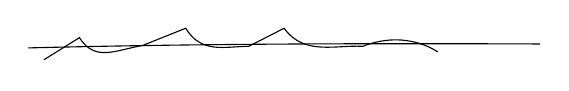
\begin{tikzpicture}[x=1cm,y=1cm]
\draw (0,0) .. controls (2,.05) and (4,.06) .. (6.5,.05);
\draw (.2,-.15) -- (.65,.13) .. controls (.85,-.18) and (1.1,-.03) .. (1.45,.03)
 -- (2,.25) .. controls (2.2,-.08) and (2.5,.02) .. (2.8,.02)
 -- (3.25,.25) .. controls (3.5,-.1) and (3.9,.04) .. (4.25,.02)
 .. controls (4.65,.18) and (5,.08) .. (5.2,-.05);
\end{tikzpicture}}

\margin{61}
